\section{ECOSYSTEM} \label{ecosystem}

We believe that the current model of Maker \& Exchange Platforms is not fair to creators and buyers and that by using decentralized systems where no central authority has control, we can build an ecosystem of tools \& services that offers creators the freedom to license \& distribute their work, while maintaining all benefits of existing traditional platforms. The BlockLicense ecosystem aims to embrace both creators and buyers and make the process of licensing \& funding extremelly simple by providing a wide range of tools specifically created for this purpose.


\subsection{The License Coin}

All transactions within the BlockLicense ecosystem take place in License Coins (LCN) (Table \ref{table:lcn}), an Ethereum based ERC20 \cite{erc20} token, enabling very fast transactions and almost instant payouts. An ecosystem-specific token is paramount to the viability of the project since its price is not affected by the fluctuations of Ether, it creates a closed ecosystem economy and it enables us to provide incentives to creators and buyers for participating in the BlockLicense Ecosystem. Also, since LCN has utilitarian value within the BlockLicense ecosystem, LCN holders will be encouraged to use BlockLicense for their licensing needs and help the community grow. Initial LCN distribution will take place through a crowdsale that is described in detail in Section \ref{crowdsale} of this document and through which we will be bootstrapping the development and promotion of the ecosystem. Once the LCN crowdsale is over, LCN will be listed in several crypto exchanges to be traded at will.

\begin{table}[t!]
\begin{center}
\begin{tabular}{c c c c c c}
& & \\ % put some space after the caption
\toprule
\textbf{Name} & \textbf{Symbol}  & \textbf{ETH Rate} & \textbf{Total Issued}  & \textbf{Decimal Points} & \textbf{Type}\\
\midrule
 License Coin & LCN & 2,000 LCN to 1 ETH & 700,000,000 LCN & 18 & ERC20\\
\bottomrule
\end{tabular}
\end{center}
\caption{License Coin Data}
\label{table:lcn}
\end{table}

\subsection{The Web Platform}

The BlockLicense Web Platform is a web-based marketplace for BlockLicense content. The Platform is the central gateway where buyers can browse submitted content and acquire licenses on digital files for their desired use-case. The Web Platform is mainly targetting buyers of digital content.

\subsection{Website Shop Widgets}
A very important part of the ecosystem are Shop Widgets that enable the embedding of shops in custom websites. Shop widgets utilize the Reseller feature of BlockLicene, by enabling buyers to act as curators of content and create lists of digital content than can be embedded and sold through their personal websites.

\subsection{The BlockLicense App}

The BlockLicense Desktop App is a cross-platform application available in all major Operating Systems (Windows, OSX, Linux) targeting both creators and buyers. It acts as a software-based LCN wallet that enables token holders to transfer Lisense Coins, view licensing information of local files that have the BlockLicense information embedded and acquire licenses for permissible uses. Creators can use the application to manage their cloud-based library of custom licenses, add BlockLicense information to their files by setting their desired licensing and pricing options and submit their content to the BlockLicense Web Platform. The Desktop Application integrates fully with the rest of the ecosystem and provides one of the main pathways users can take to produce and consume BlockLicense content.

\subsection{Design Software Plugins}

With BlockLicense we aim to make the process of setting licensing \& pricing information very simple and make sure it does not add significant work to creators. By creating BlockLicense plugins for popular design software such as ones created by Adobe \cite{adobe}, we aim to make the process of licensing an integral part of the creators workflow, all within a familiar environment. Complex tasks such as optimal pricing determination can be greatly simplified by providing usefull feedback to creators such as the average price of similar work and the price of bestseller items within the ecosystem. Design software plugins integrate with the rest of the ecosystem and allow creators to set their licensing \& pricing options and make their files available within the Web Platform.



\subsection{Mobile App}

The BlockLicense MobileApp provides tools for submitting time-sensitive content such as footage \& photos of events that are newsworthy. It connects people on the streets with newsrooms and integrates with the Web Platform so that news networks can acquire licenses for their desired content. It enables citizen journalists to sell their content and provides breaking news videos \& photos to news networks.


\subsection{BlockLicense Architecture}

The BlockLicense Architecture utilizes decentralized services for the core functionality of the system, enforcing the longevity of submitted data while decoupling the availability of services from BlockLicense success. The Ethereum blockchain and Virtual Machine are used for the verification of all BlockLicense metadata attached to a file and for all payment processing and routing needs as specified by the creator. IPFS \cite{ipfs} is used for storage of binary files while BigchainDB \cite{bigchaindb} is used for all database related needs of the ecosystem.

\begin{figure}[h]
\centering
\begin{minipage}{1\textwidth}
  \centering
  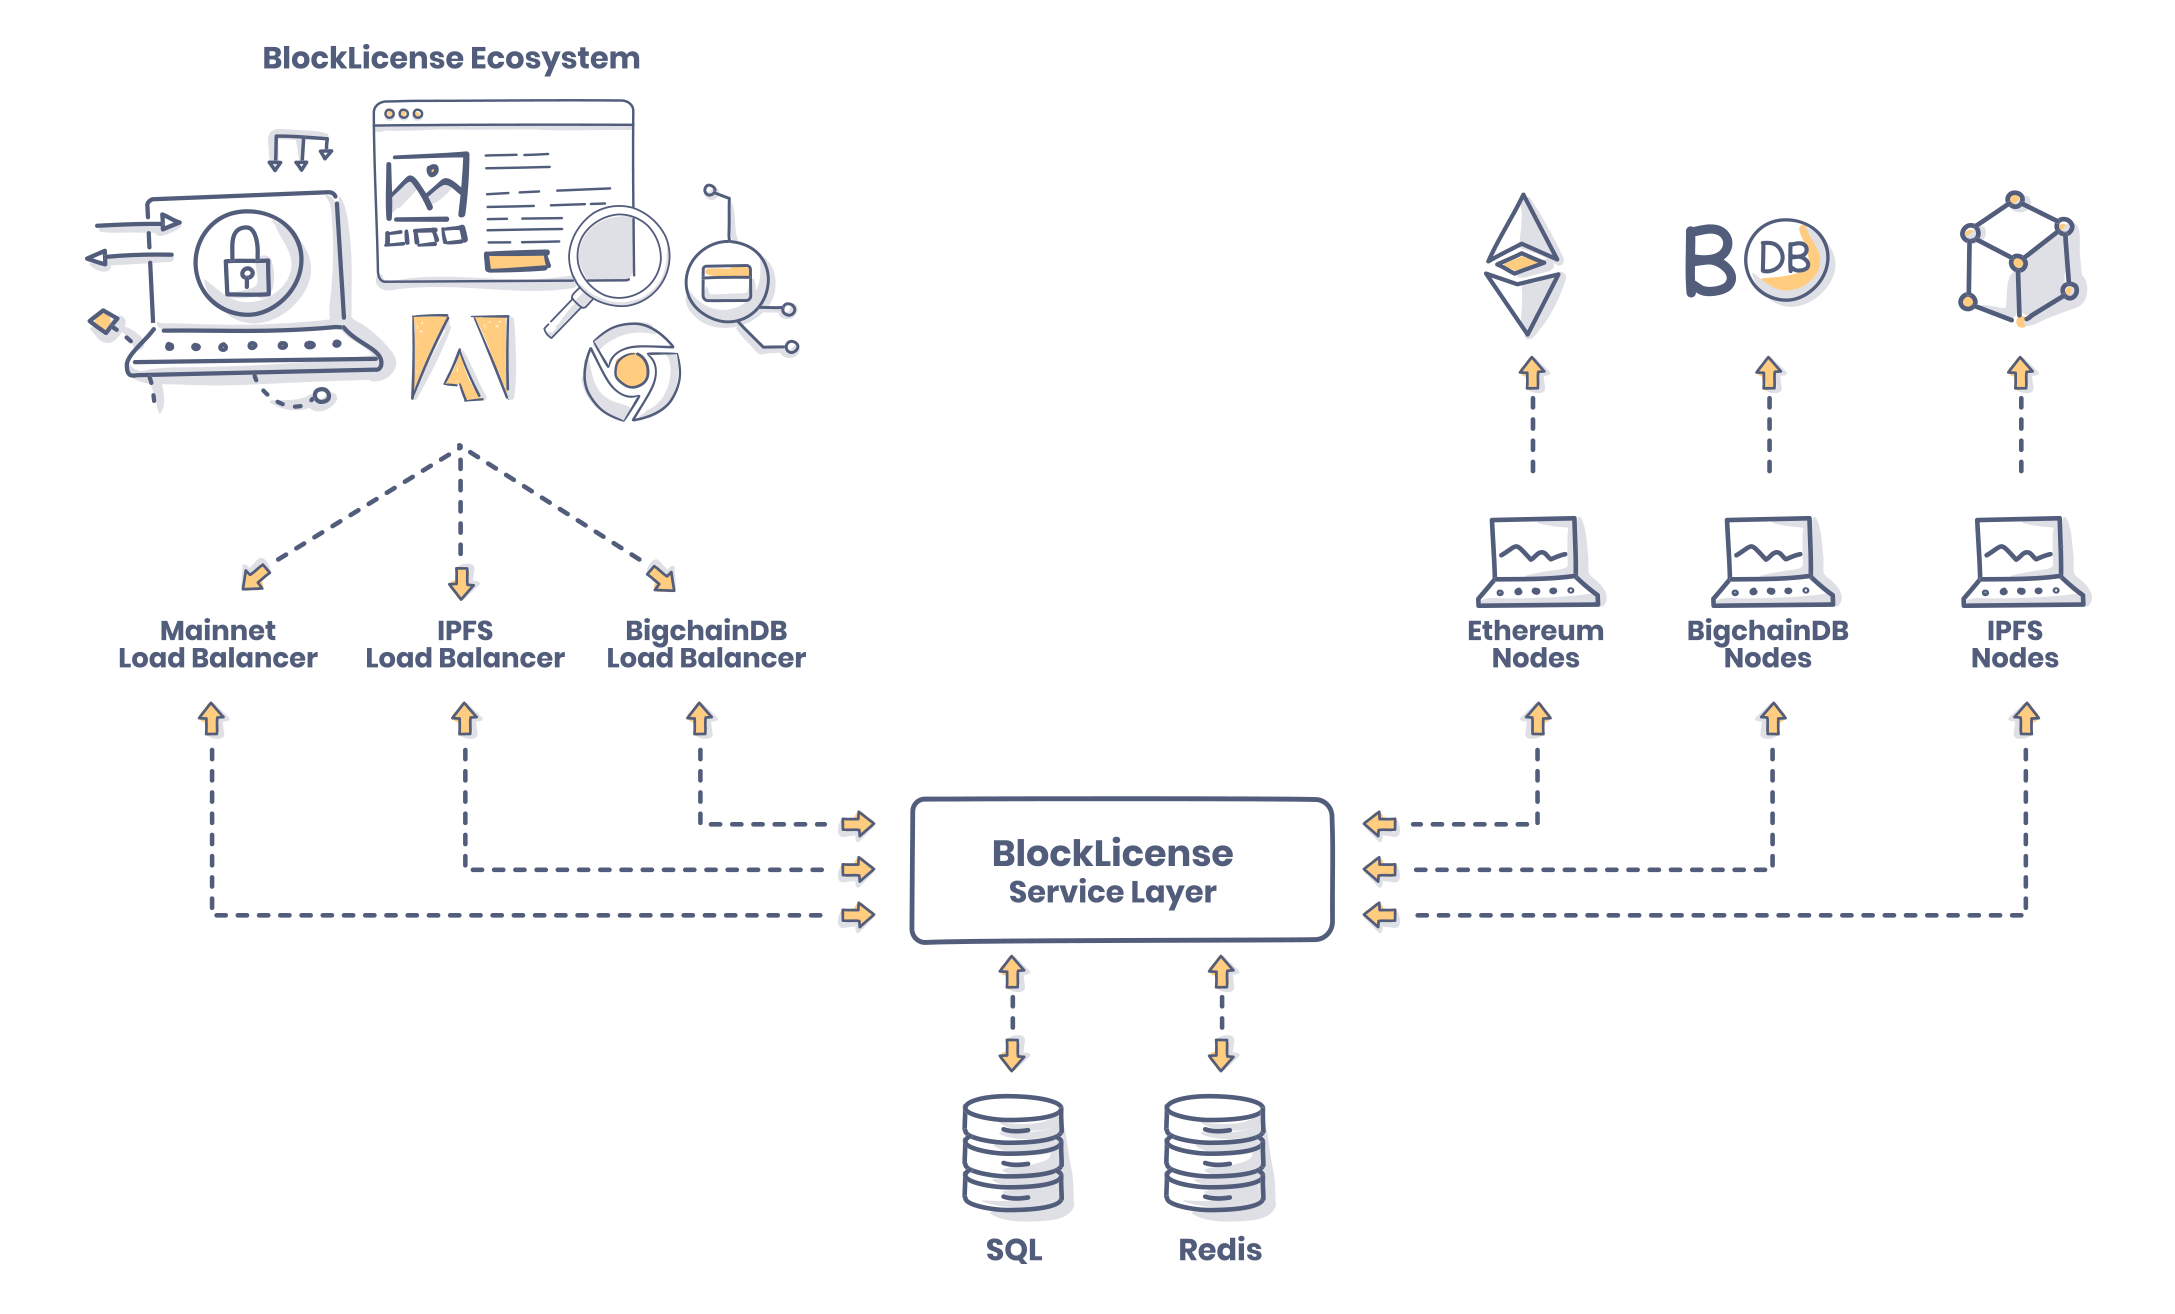
\includegraphics[width=1\linewidth]{./figures/fig7.png}
  \caption{BlockLicense System Architecture.}
  \label{fig:system}
\end{minipage}%
\end{figure}
